\section{Additional Theoretical ICD/ETMD3 Spectra}

\subsection{Clusters with $N=38$ Atoms of Different Composition}
Recently, structures for ArXe clusters of in total 38 atoms were optimized
using an evolutionary algorithm based on two-body potentials determined
by xyz. \cite{}
In this section, the simulated ICD and ETMD3 spectra for selected cluster
structures shown in Figure xyz of Ref. \citenum{} are shown in Figures
\ref{} -- \ref{} and discussed.


\begin{figure}
 \centering
 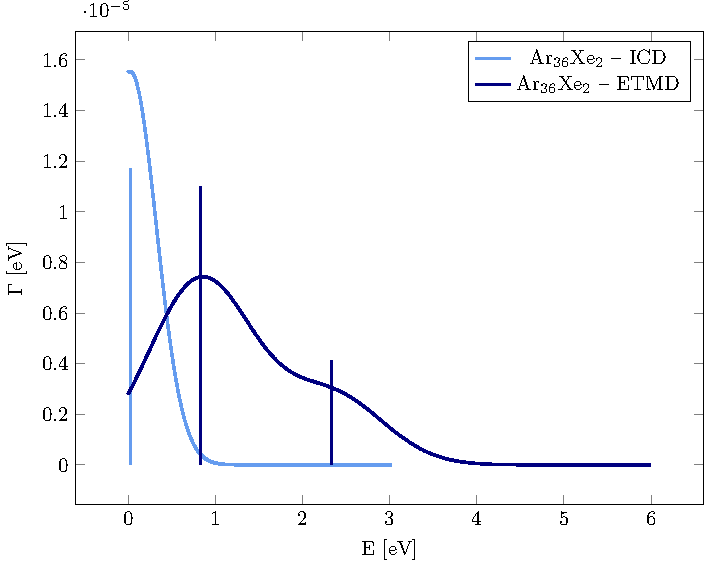
\includegraphics[width=0.5\columnwidth]{pics/Ar36Xe2.pdf}
 \caption{}
 \label{}
\end{figure}


\begin{figure}
 \centering
 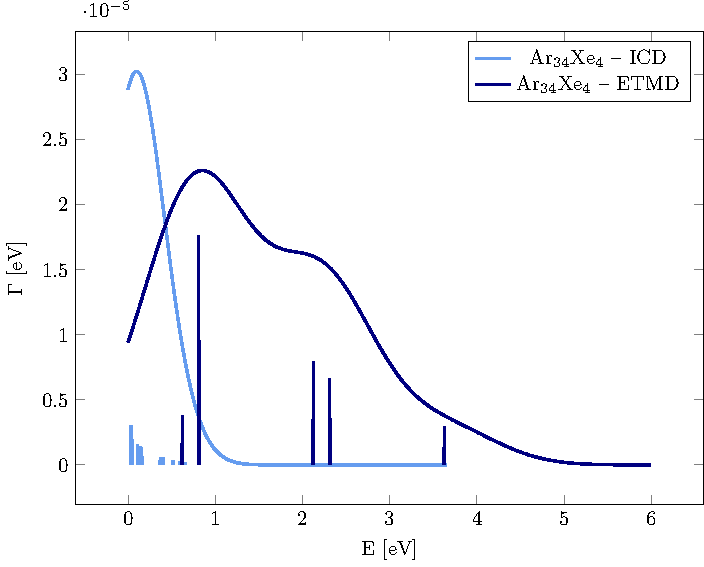
\includegraphics[width=0.5\columnwidth]{pics/Ar34Xe4.pdf}
 \caption{}
 \label{}
\end{figure}


\begin{figure}
 \centering
 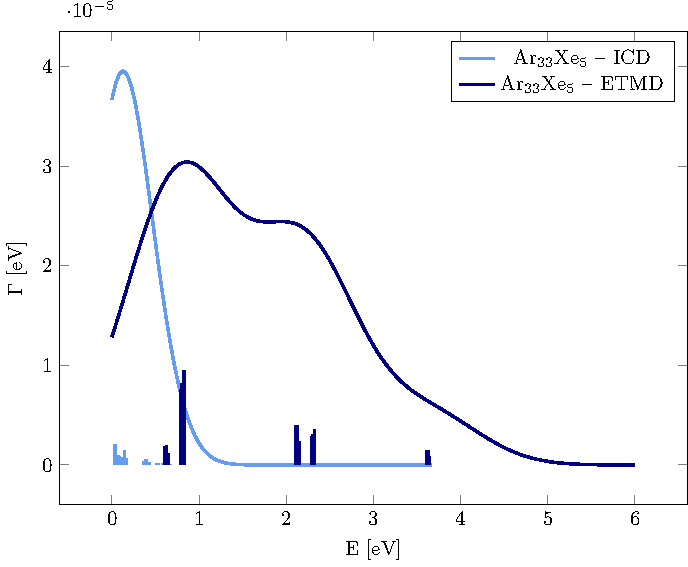
\includegraphics[width=0.5\columnwidth]{pics/Ar33Xe5.pdf}
 \caption{}
 \label{}
\end{figure}

\begin{figure}
 \centering
 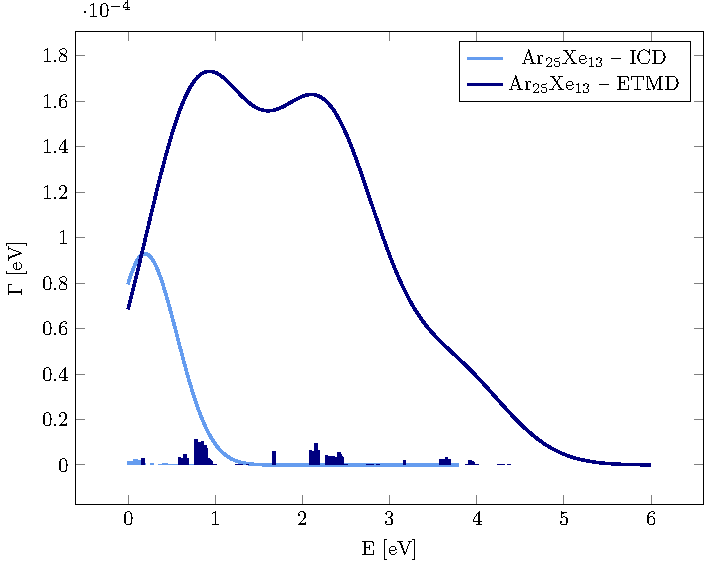
\includegraphics[width=0.5\columnwidth]{pics/Ar25Xe13.pdf}
 \caption{}
 \label{}
\end{figure}

\begin{figure}
 \centering
 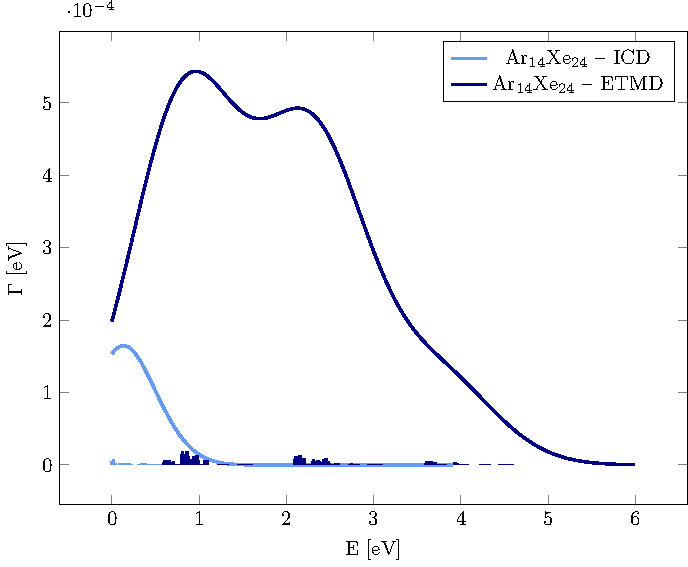
\includegraphics[width=0.5\columnwidth]{pics/Ar14Xe24.pdf}
 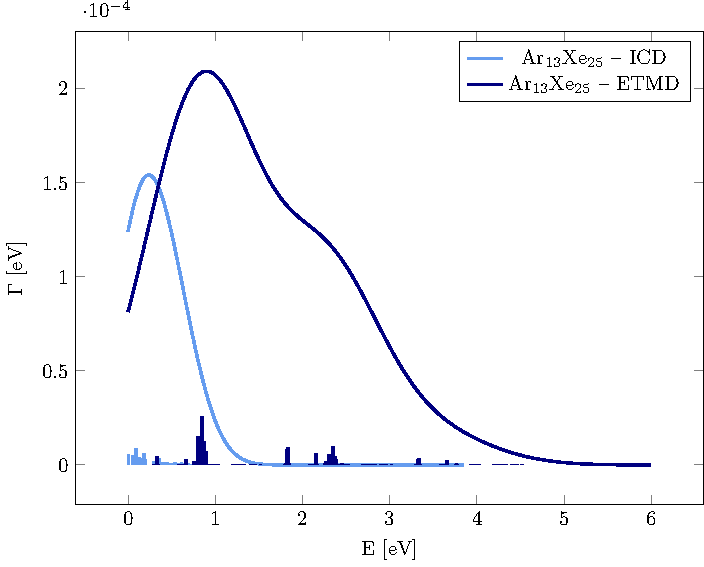
\includegraphics[width=0.5\columnwidth]{pics/Ar13Xe25.pdf}
 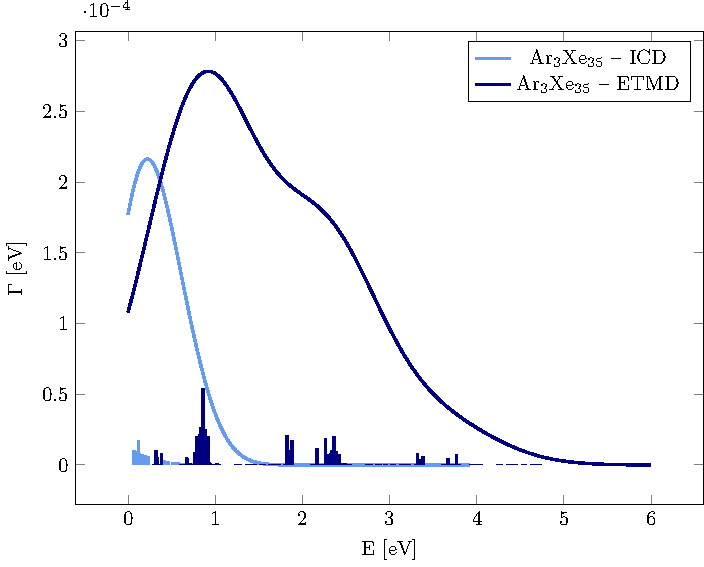
\includegraphics[width=0.5\columnwidth]{pics/Ar3Xe35.pdf}
 \caption{Ar$_x$Xe$_y$ clusters with a xenon content of more than \unit[50]{\%}.
          The ETMD3 is the dominant processi for these cluster structures.
          They are shown for completeness but can, due to the high xenon content,
          not be related to the experimental secondary electron measurements.}
 \label{figure:ArXe_gt50}
\end{figure}


For all these cluster structures the ETMD3 is the more probable decay process and
except for the Ar$_{36}$Xe$_2$ case with \unit[43.6]{\%} ICD, the ETMD3 is clearly
the dominant process (compare Table xyz of the main article).
This can be explained by a combination of high xenon content and the
scattered distribution of the xenon atoms within the cluster structures.
Since the decay width of the ETMD3 is mostly caused by the decay
with direct neighbours and for these $\Gamma_{ETMD3} \propto N_{Ar} N_{Xe}^2$
both the maximization of direct xenon neighbours of an argon atom and the
maximization of the number of argon atoms being surrounded by xenon atoms
leads to a strong increase of the ETMD3 decay width. This situation is realized
in cluster structures without a seggregation of the two different elements like
in the structures of Ref. \cite{}. At the same time, all ICD channels are closed
for direct xenon neighbours. Therefore, a higher number of direct xenon neighbours
for all argon atoms reduces the number of possible decay partners for a given
cluster composition and therefore the ICD decay width.



%\begin{figure}
% \centering
% \includegraphics[width=0.5\columnwidth]{pics/ArXe.pdf}
% \caption{}
% \label{}
%\end{figure}
%
%\begin{figure}
% \centering
% \includegraphics[width=0.5\columnwidth]{pics/ArXe.pdf}
% \caption{}
% \label{}
%\end{figure}
